\documentclass[10pt,twocolumn,letterpaper,english]{article}

%%%%%%%%% PAPER TYPE  - PLEASE UPDATE FOR FINAL VERSION
%\usepackage[review]{cvpr}      % To produce the REVIEW version
\usepackage{cvpr}              % To produce the CAMERA-READY version
%\usepackage[pagenumbers]{cvpr} % To force page numbers, e.g. for an arXiv version

% Include other packages here, before hyperref.
\usepackage{xurl}
\usepackage{graphicx}
\usepackage{amsmath}
\usepackage{amssymb}
\usepackage{booktabs}

\usepackage{enumitem}
\setlist[itemize]{noitemsep, topsep=0pt}

% It is strongly recommended to use hyperref, especially for the review version.
% hyperref with option pagebackref eases the reviewers' job.
% Please disable hyperref *only* if you encounter grave issues, e.g. with the
% file validation for the camera-ready version.
%
% If you comment hyperref and then uncomment it, you should delete
% ReviewTempalte.aux before re-running LaTeX.
% (Or just hit 'q' on the first LaTeX run, let it finish, and you
%  should be clear).
\usepackage[pagebackref,breaklinks,colorlinks]{hyperref}


% Support for easy cross-referencing
\usepackage[capitalize]{cleveref}
\crefname{section}{Sec.}{Secs.}
\Crefname{section}{Section}{Sections}
\Crefname{table}{Table}{Tables}
\crefname{table}{Tab.}{Tabs.}

\title{Remote Cross-Platform Collaboration -- Final Report}
\author{Valentin Ogier \qquad Agostino Nickl \qquad Andrea Settimi \qquad Wenqian Yang \\ ETH Zürich, Switzerland}
%\date{November 2021}

%%%%%%%%% PAPER ID  - PLEASE UPDATE
\def\cvprPaperID{*****} % *** Enter the CVPR Paper ID here
\def\confName{CVPR}
\def\confYear{2022}

\bibliographystyle{plain}

\begin{document}

\maketitle

\section{Abstract}

This project deals with remote, cross-platform collaboration scenarios between Augmented Reality (AR) and Virtual Reality (VR), as required for maintenance, construction or training purposes. Despite maturing hardware and software solutions and interoperability standards, pilot applications and documentation in this field are sparse. As part of this project, we have built a prototypical application that works across an AR headset (the Microsoft Hololens 2) and a VR headset (the HTC Vive Pro) to demonstrate the possibility of such a shared work environment. In this report, we will write about the critical features of our design and the main challenges we encountered, and continue with an evaluation of two test runs conducted building a chair with AR instructions shared remotely from an instructor wearing a VR headset (see \cref{sec:demo_vid}).

\section{Introduction}

\begin{figure}[!htp]
    \centering
    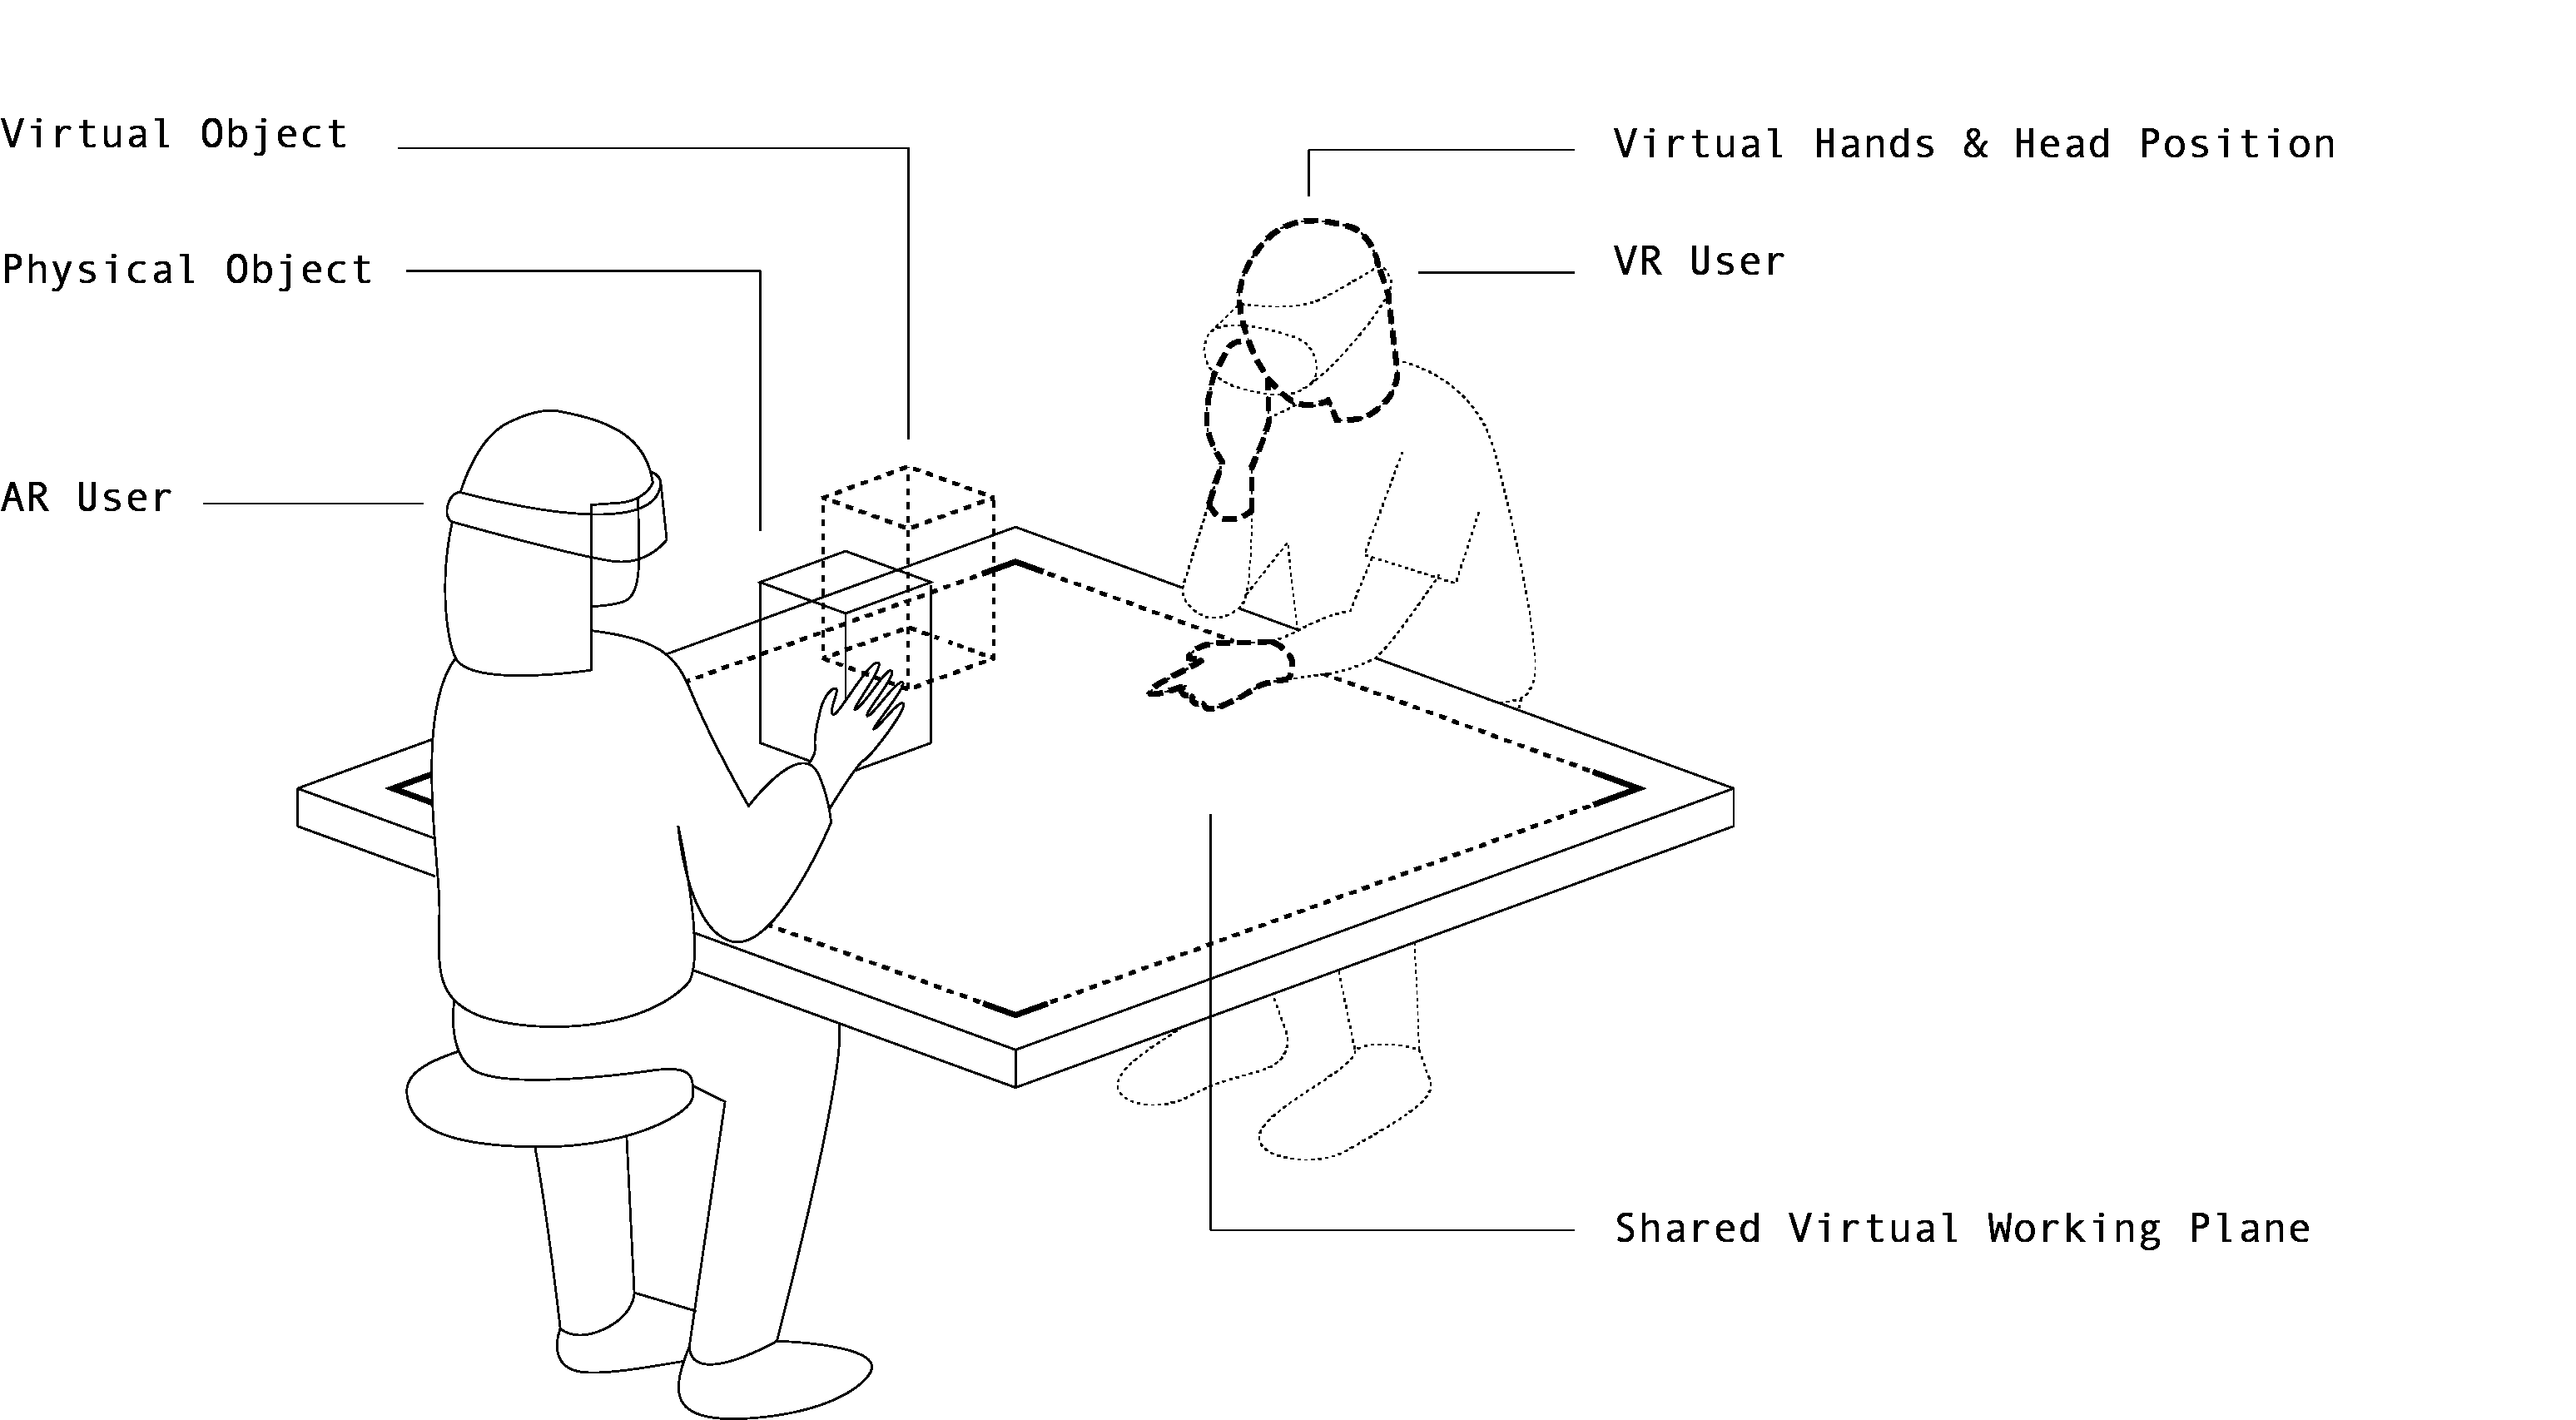
\includegraphics[width=1\linewidth]{VR_20Proposal.png}
    \caption{Early Design Schematic. Drawing by the authors.}
    \label{fig:Vr Proposal}
\end{figure}

Our project aims to allow a Virtual Reality (VR) user and an Augmented Reality (AR) user–-joining from different locations and platforms-–to participate in a shared, Mixed Reality (MR) work environment. In this virtual environment, they can see each other's avatars consisting of head and hand positions, speak to each other, and share virtual objects on a common work plane (see \cref{fig:Vr Proposal}). 

Key use cases include giving intuitive, spatialized instructions without participants having to be located in the same room. For example, one user might be completely virtually immersed in a VR environment in one room, while the AR user is located in a different room where he will carry out a task, e.g.\ building a chair in a workshop.

\subsection{Motivation}

Applications allowing multiple users to access a shared virtual space over the internet from identical or varying immersive platforms, e.g.\ VR and PC, have received an increasing amount of attention in the last years, especially in the context of the pandemic, and are by now well documented. Prominent applications include platforms like VR Chat or Mozilla Hubs. In the past years, ``serious'' use cases for MR applications in industry and manufacturing sectors gained more attention \cite{augmentedrealityinproduction}, and the discussion around the interoperability and immersion levels of a ``Metaverse'' picked up steam \cite{metaverse}.

However, research on cross-platform collaboration between AR and VR has received little attention, and pilot projects bridging different platforms, standards, and input definitions are yet few and far between (see \cref{sec:prior_work}).

This research project aims to bridge this gap, making use of three recent innovations that help enable cross-platform MR applications. MRTK\cite{polar-kevMRTKUnityDeveloperDocumentation}, developed by Microsoft, is a toolkit that makes designing interactions for the Hololens 2 and other AR/VR devices easier. OpenXR\cite{OpenXR} is a maturing standard allowing to build MR applications compatible with a wide range of headsets (AR and VR) and controllers. Finally, Photon Unity Networking (PUN2)\cite{PhotonUnity3D}, developed by Exit Games, promises robust networking solutions for multiplayer games.

\subsection{Main Contribution}

\begin{figure}[!htp]
    \centering
    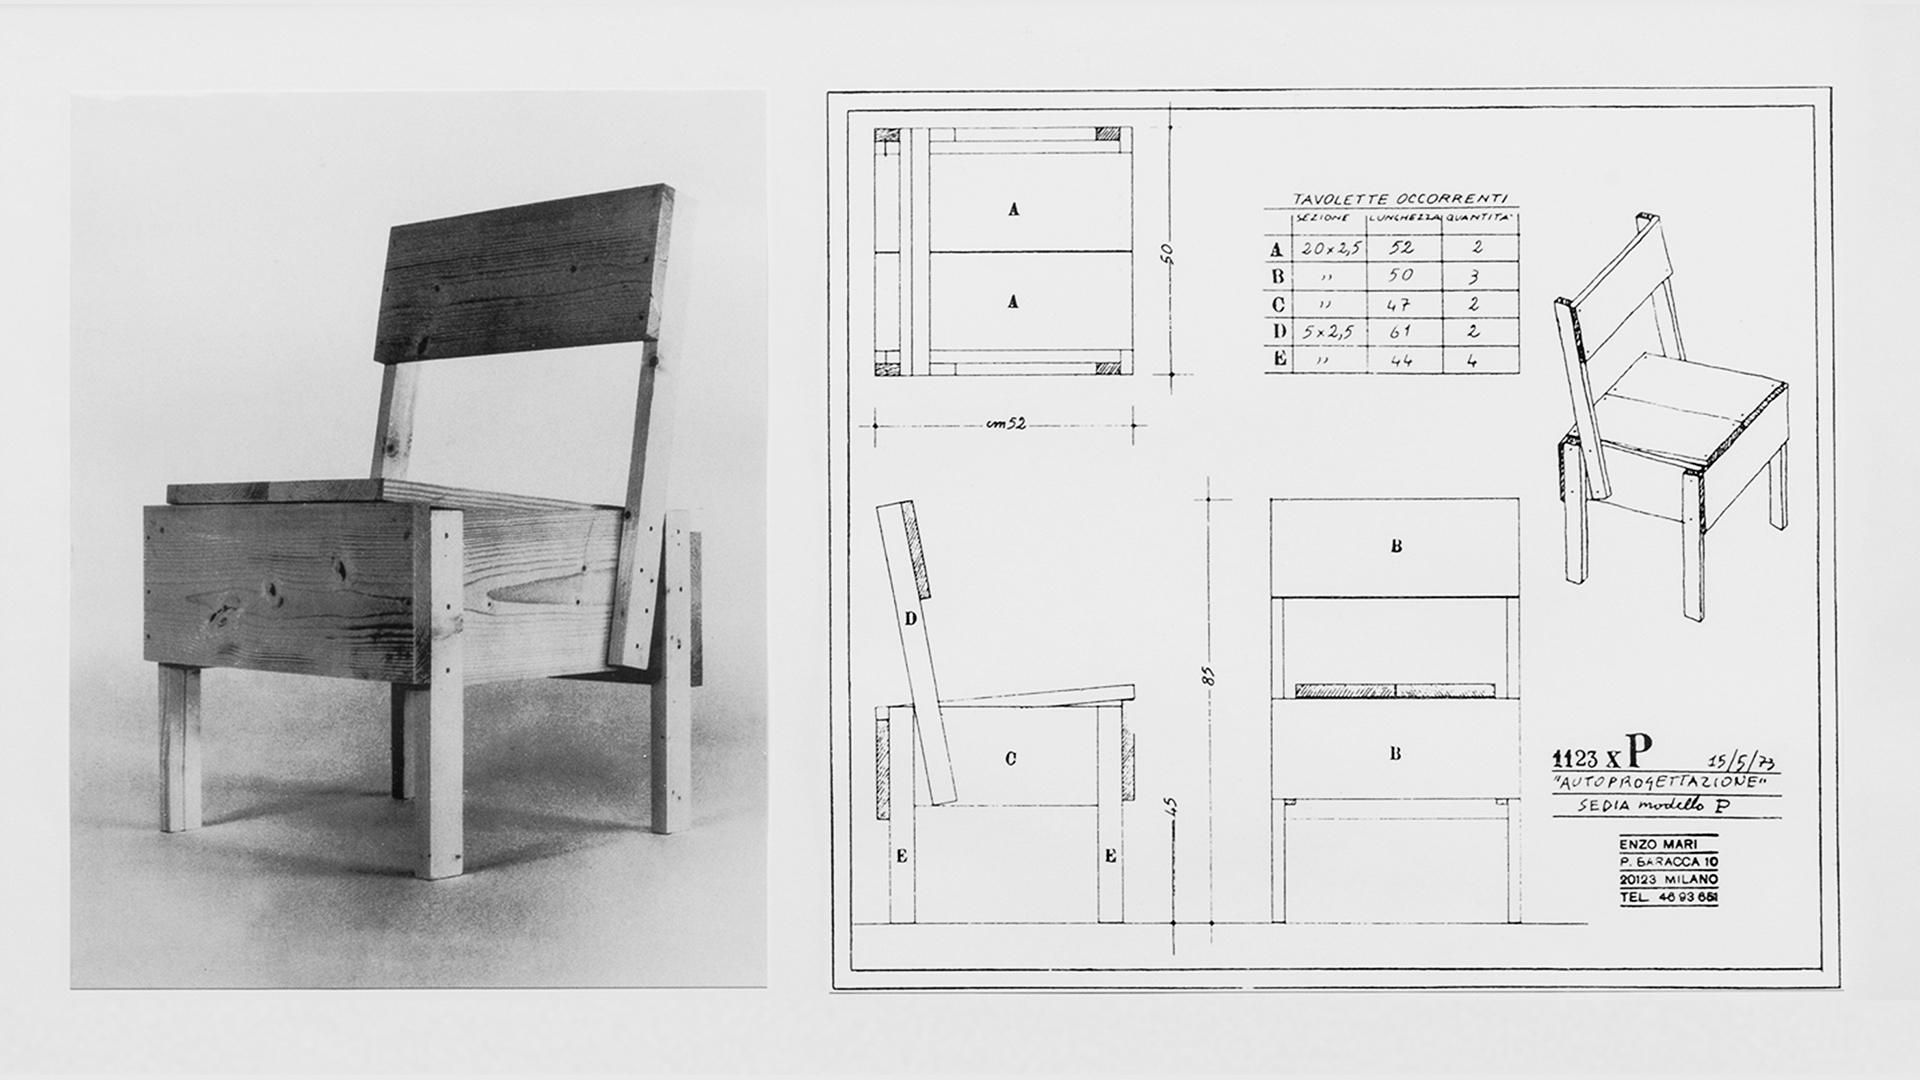
\includegraphics[width=1\linewidth]{3_Enzo-Mari.jpg}
    \caption{Construction drawings of Sedia 1 by Enzo Mari. Image source: \url{salonemilano.it}.}
    \label{fig:sedia1}
\end{figure}

\begin{figure}[!htp]
    \centering
    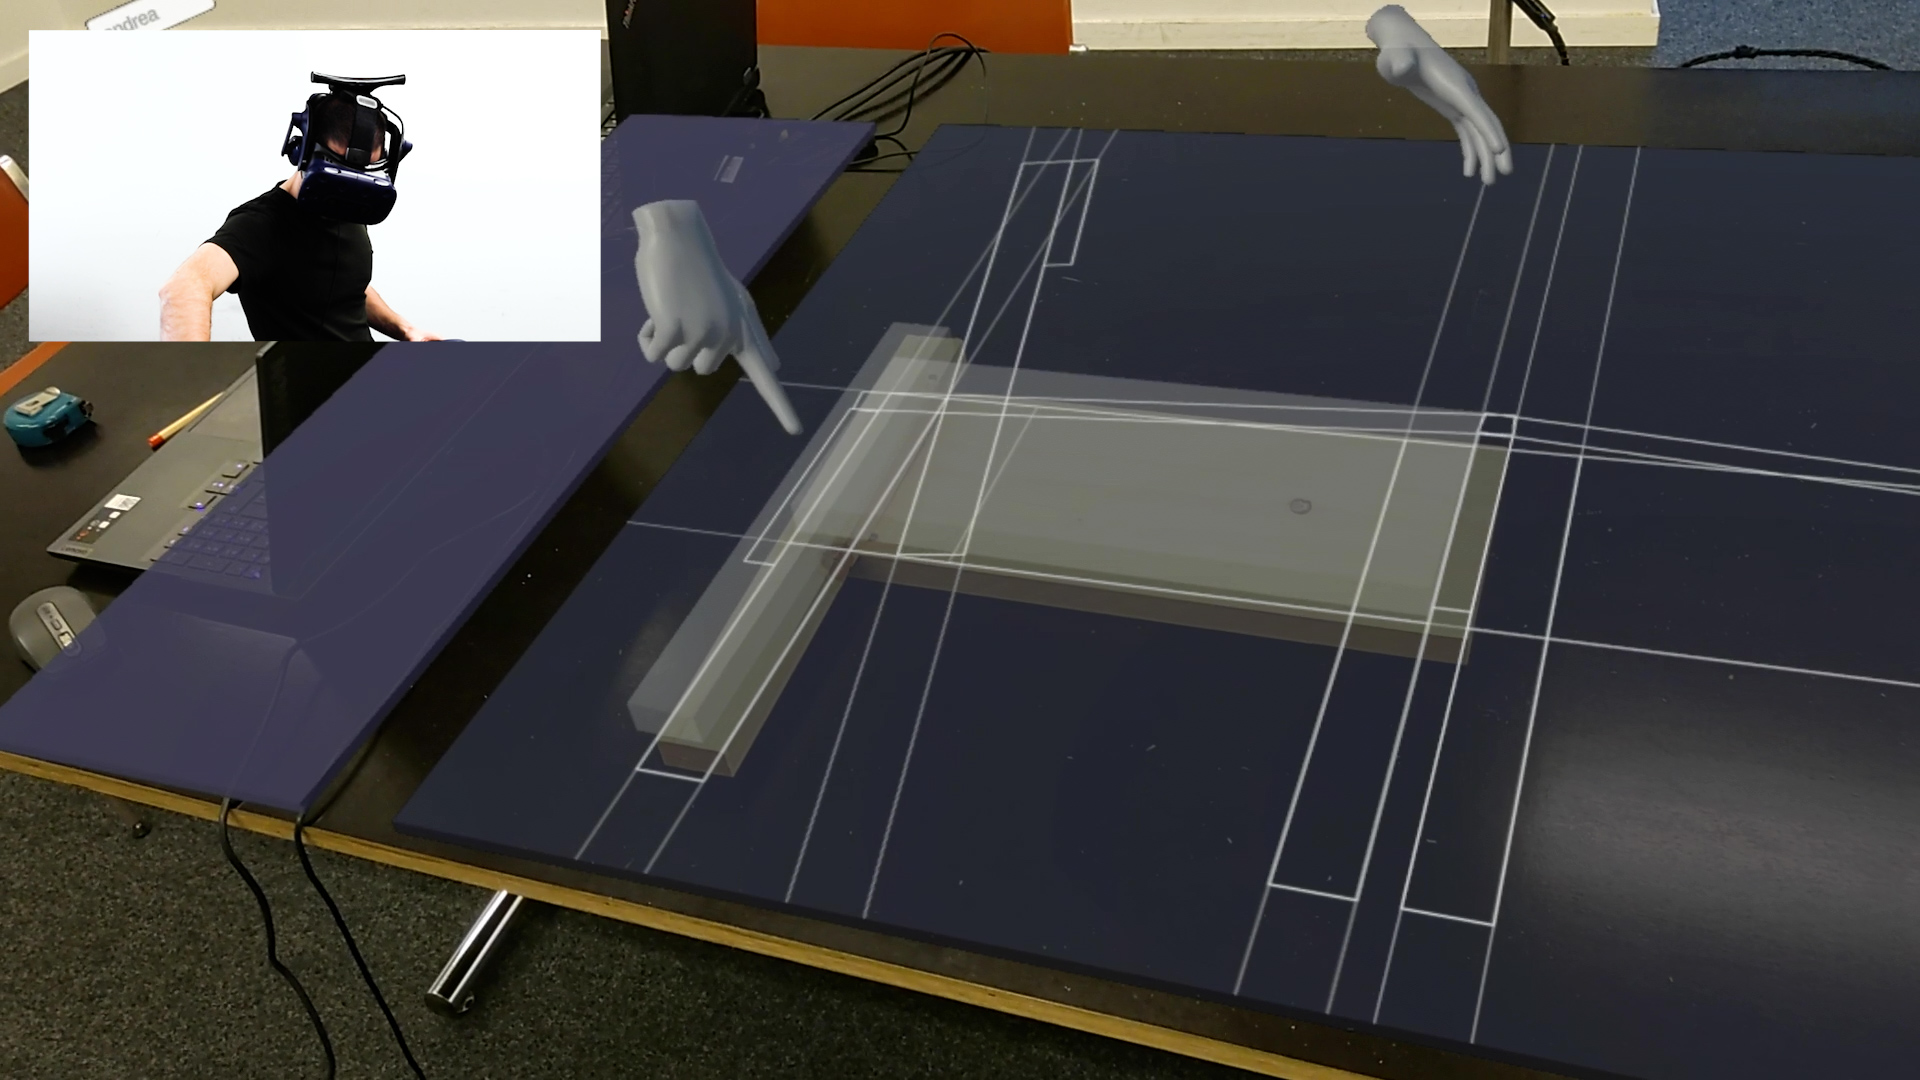
\includegraphics[width=1\linewidth]{Pointers.jpg}
    \caption{A remotely located VR user giving instructions. Image by the authors.}
    \label{fig:VR_user}
\end{figure}

\begin{figure}[!htp]
    \centering
    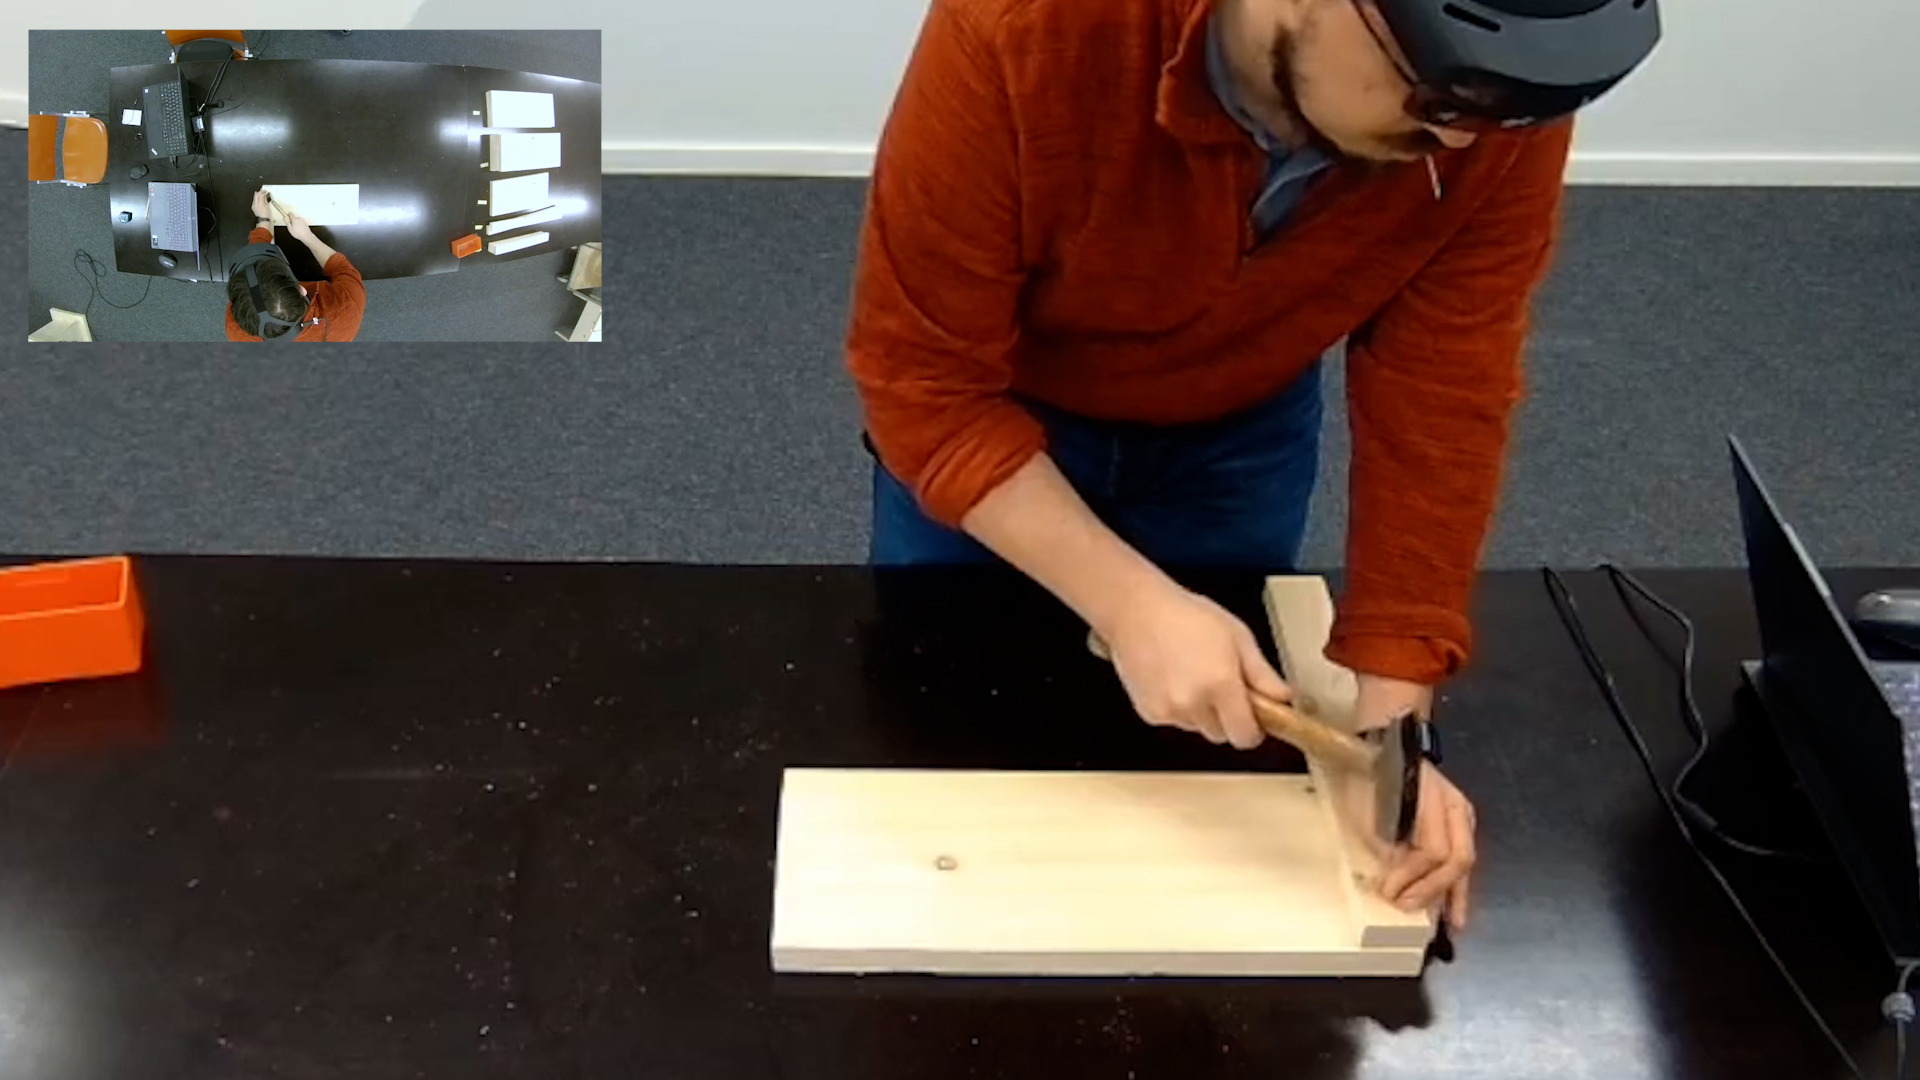
\includegraphics[width=1\linewidth]{Hololens.jpg}
    \caption{The AR user follows instructions in a workshop. Image by the authors.}
    \label{fig:AR_user}
\end{figure}

Built with Unity, our resulting pilot application runs on both the Microsoft Hololens 2 and the HTC Vive Pro headset. In a shared (immersive or augmented) workplace, users can see each other's avatars consisting of head and hand positions, speak to each other, and share virtual objects on a common work plane to remotely collaborate in building virtual and physical assemblages.

In order to test our application with an exemplary use case, we chose to collaboratively build a 1974 Design Classic, Sedia 1 by Enzo Mari. The design requires 13 pre-cut timber pieces of varying dimensions, all of which are nailed together in the construction process. Instead of building it with the original, paper construction drawings \cref{fig:sedia1}), one participant takes the role of the VR instructor (see \cref{fig:VR_user}), guiding a remote trainee (see \cref{fig:AR_user})--unfamiliar with the design, but equipped with an AR headset–-through every step of construction by demonstrating it on a digital twin. The VR instructor manipulates virtual elements representing the chair parts to guide the trainee. These parts are shown to the trainee as holograms overlaying his immediate surroundings, guiding him as he manipulate the real chair parts and nails them together.

In the following, we will describe the key features of the remote cross-platform collaboration pilot application, as well as insights stemming from the technical and design development process. In lack of a designated user study, we will share our impressions on usability collected during two extensive rounds of testing of the app, building one chair each round.

\section{Prior Work}\label{sec:prior_work}

It is no surprise that AR technologies have been first employed in tasks where robots could not perform at their best or are still facing critical challenges. In-situ additive construction is one of those tasks. From holographic models deployed as augmented 3D templates with Hololens 1 and 2 \cite{holographicconstruction}, we assisted in the development of newly computed feedback loop logics to guide the operators \cite{objectbasedvisualinertia}. Strong of these previous works and antecedent researches on in-situ robotic assembly \cite{autoreposition, kinematic}, systems like the one deployed in ``Augmented acoustics'' \cite{augmentedacoustics} and later in ``Augmented bricklaying'' \cite{augmentedbricklaying} have shown the potential to seamlessly track physical element position and inform the augmented framework about the updated as-built context at the scale of a real building site. Recently, the start-up incon.ai \cite{incon} has implemented such systems into a commercial application that can automatically generate building plans from CAD models and display them as augmented instructions on multiple interfaces. With such a new generation of AR construction systems, we are starting to witness realizations with qualities and precision levels that were before unachievable if not by elaborate robotic aggregation. Besides augmented machine-guided operations, collaborative MR systems represent an alternative that has mainly been adopted in industrial tasks involving maintenance, repair and assembly. One of the earliest systems offers assistance in aircraft wire bundles operations \cite{caudell1992augmented}. Since then, latency on long-distance data-transfer has consistently improved, boosting the development of MR remote assistance systems \cite{zhong2002collaborative, chen2013semarbeta}. Tele-assistance was early designed to allow skilled operators to assist un-trained ones thanks to camera streams mounted on the AR device \cite{bottecchia2010tac}. Smart assembly procedures were also developed and tested in real scenarios of maintenance tasks \cite{mourtzis2016cloud}. Recently, researchers have shown that it is possible to add immersiveness to remotely guided tasks by visualizing the working space and providing assistance in 3D coordinates \cite{wang2014augmented, yin2020vr}.


\section{Methodology}

In the following, we will speak about the equipment used, as well as key technical and design features of our application in more detail.

\subsection{Hardware and Software Equipment}

We use two different kinds of Head-Mounted-Displays (HMDs) for our project (see \cref{fig:hmd}). The Microsoft Hololens 2 is the most advanced, commercially available, stand-alone AR headset, allowing users to project holograms on their immediate, physical environment. The HTC Vive Pro is a VR headset with six degrees of freedom, often used for tasks requiring high precision in movements and resolution, e.g.\ gaming applications. Content is streamed from a local computer. The HTC Vive Pro requires stationary tracking and uses controllers as inputs.

\begin{figure}[!htp]
    \centering
    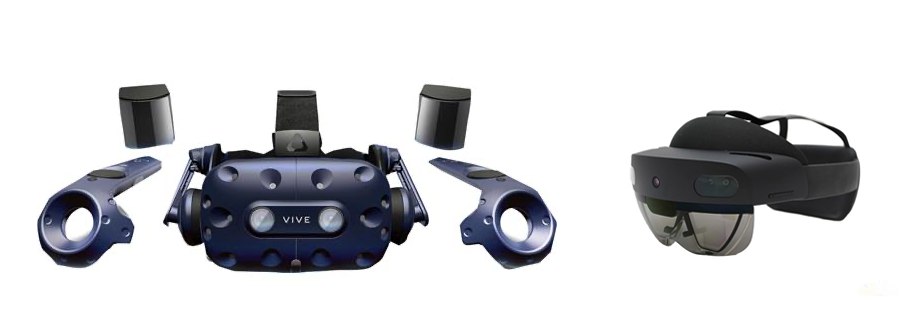
\includegraphics[width=1\linewidth]{headsets.png}
    \caption{We use the HTC Vive Pro (left) as VR headset and the Microsoft Hololens 2 (right) as AR headset. Image sources: \url{virtualrealityhire.com} and \url{techmania.ch}.}
    \label{fig:hmd}
\end{figure}

These two platforms constitute the target devices for our project. The main engine we chose to develop with is Unity: As a general-purpose game engine, it provides functionalities commonly used in 3D applications, like 3D rendering, physics simulation, and programmable behaviors via scripting. It does not, however, deal with the specificities of AR/VR devices: hand and head tracking, eye tracking and spatial awareness on the Hololens 2, and tracking of the controllers on the HTC Vive for instance. To bridge the gap between the input system provided by Unity and the information made available by the HMDs, the vendors provide APIs and runtime libraries. As recently as early 2021, the different devices used different libraries (Windows Mixed Reality for the Hololens 2, OpenVR for the HTC Vive): In this situation, it was necessary to develop two different Unity applications to target the two devices. However, a recent initiative called OpenXR has led to the creation of a common set of APIs and runtime libraries for a large range of AR/VR devices: In the course of 2021, both the Hololens 2 and the HTC Vive Pro have been made compatible with the OpenXR standard. With the right Unity configuration, it has therefore been possible for us to develop a single application targeting both devices.

In order to quickly build a full-fledged application, our project relies on two powerful Unity libraries. The first one, Microsoft's Mixed Reality Toolkit (MRTK), gives access to a number of components making it easy to add spatial interaction. The second one, Photon Unity Networking 2 (PUN2), makes it possible to synchronize the state (e.g.\ position and rotation) of elements between several users regardless of the HMD they use, and provides other lower-level network primitives. 

It should be noted here that parts of this infrastructure are still under heavy development (as is the case for most AR/VR libraries). On the one hand, this caused our experience as developers to sometimes be hindered by bugs in the libraries; on the other, it led to very quick answers by the project maintainers. We reported one bug and contributed to the discussion of another one on the MRTK project's issue tracker, one of which was linked to our use of the OpenXR deployment target\footnote{Issues number \href{https://github.com/microsoft/MixedRealityToolkit-Unity/issues/10297}{\#10297} and \href{https://github.com/microsoft/MixedRealityToolkit-Unity/issues/10347}{\#10347} on \url{https://github.com/microsoft/MixedRealityToolkit-Unity/}.}.


\subsection{Collaboration Platforms}

For each team member to work on the same file, we adopted Unity Collaborate, an add-on for Unity that provides version control and synchronization for a shared project. Although a more classical GitHub version control system seems more practical for the C\# scripts present in the Unity project, Unity Collaborate offers the functionality to synchronize all modifications to objects in the scene across multiple users and proved sufficient for the collaborative development of the project.

\subsection{Network Infrastructure} 

The application we developed follows a peer-to-peer network topology (as opposed to the client-server topology commonly found in multiplayer games)\footnote{In practice, the peer-to-peer topology provided by PUN2 does use a central server for performance reasons: Data is stored on and propagated from the central server, thus requiring one connection per user with the server, instead of one connection per pair of users. The interfaces provided, however, make the presence of this server invisible to the application developer.}. This choice was made because it greatly simplifies development: A single code base is used, and every device participating in the network runs the exact same program. The number of users who can simultaneously participate in a common cooperation task is only bounded by the limits imposed by the free PUN2 plan, currently set to 20 concurrent users.

In a client-server topology, the server stores the state (e.g.\ position and rotation) of all the elements in the scene, sends the state of an element to clients when they need it, and updates the state of an element when an (authorized) client requests it. In a peer-to-peer topology, the state of the elements is spread on the different devices participating in the network. Each element is owned by a single user; meaning that a single user (called the owner) controls the shared state of this element, such as its position. The ownership can be transferred from one user to another, thus making it possible for the second user to modify the shared state of the element.

In order to make interactions feel natural, the transfer of ownership was automated: Any user can interact with any object in the scene (that is not already being interacted with) and modify its state, automatically taking ownership in the process. This automation was made possible by coordinating MRTK concepts (i.e.\ hand interaction) with PUN2 concepts (i.e.\ ownership).

\subsection{Avatars and Voice Chat}

\begin{figure}[!htp]
    \centering
    \includegraphics[width=1\linewidth]{VR:AR.jpg}
    \caption{Avatars consist of heads, hands and nametag. Image by the authors.}
    \label{fig:Vr Avatar}
\end{figure}

To create a sense of co-presence, avatars representing the users are a key requirement for collaborative MR experiences and our application. Whilst possibilities for customization in commercial applications, such as VRChat, are extensive, we left the options limited. The avatars in our application consist of an abstract, monochrome head shape and articulated hands, mimicking head and hand movements of the users, as well as optionally displaying a user's name that can be inputted through the UI menu (see \cref{fig:Vr Avatar}). 

Both HMDs are spawning in the same shared scene. The head height is used as a reference point when the scene starts to account for the different origins in the coordinate systems used by the two kinds of devices. We encountered a set of challenges concerning the initial location of the HTC Vive. We solved this problem by forcing the VR headset to the same spawning position as the Hololens 2.

In addition to the position and rotation providers of the HMDs, the hand tracking functionality of the Hololens 2 or the Vive controllers are used as input sources. The data collected is then synchronized over the network using PUN2, and the hand information is fed into modified MRTK hand visualizers to display skinned hands animated down to the joint level.

Another indispensable feature for natural communication is a low-latency voice chat. It can be implemented with an additional Unity asset by PUN2. Although the voice chat asset is free and functioning across multiple VR devices, the Hololens 2 build does need a commercial version to build and deploy on the HMD. After requesting an academic licence from Photon for the project's duration, we could also integrate the voice chat functionality for the Hololens 2.

\subsection{User Interface and Work Environment}

\begin{figure}[!htp]
    \centering
    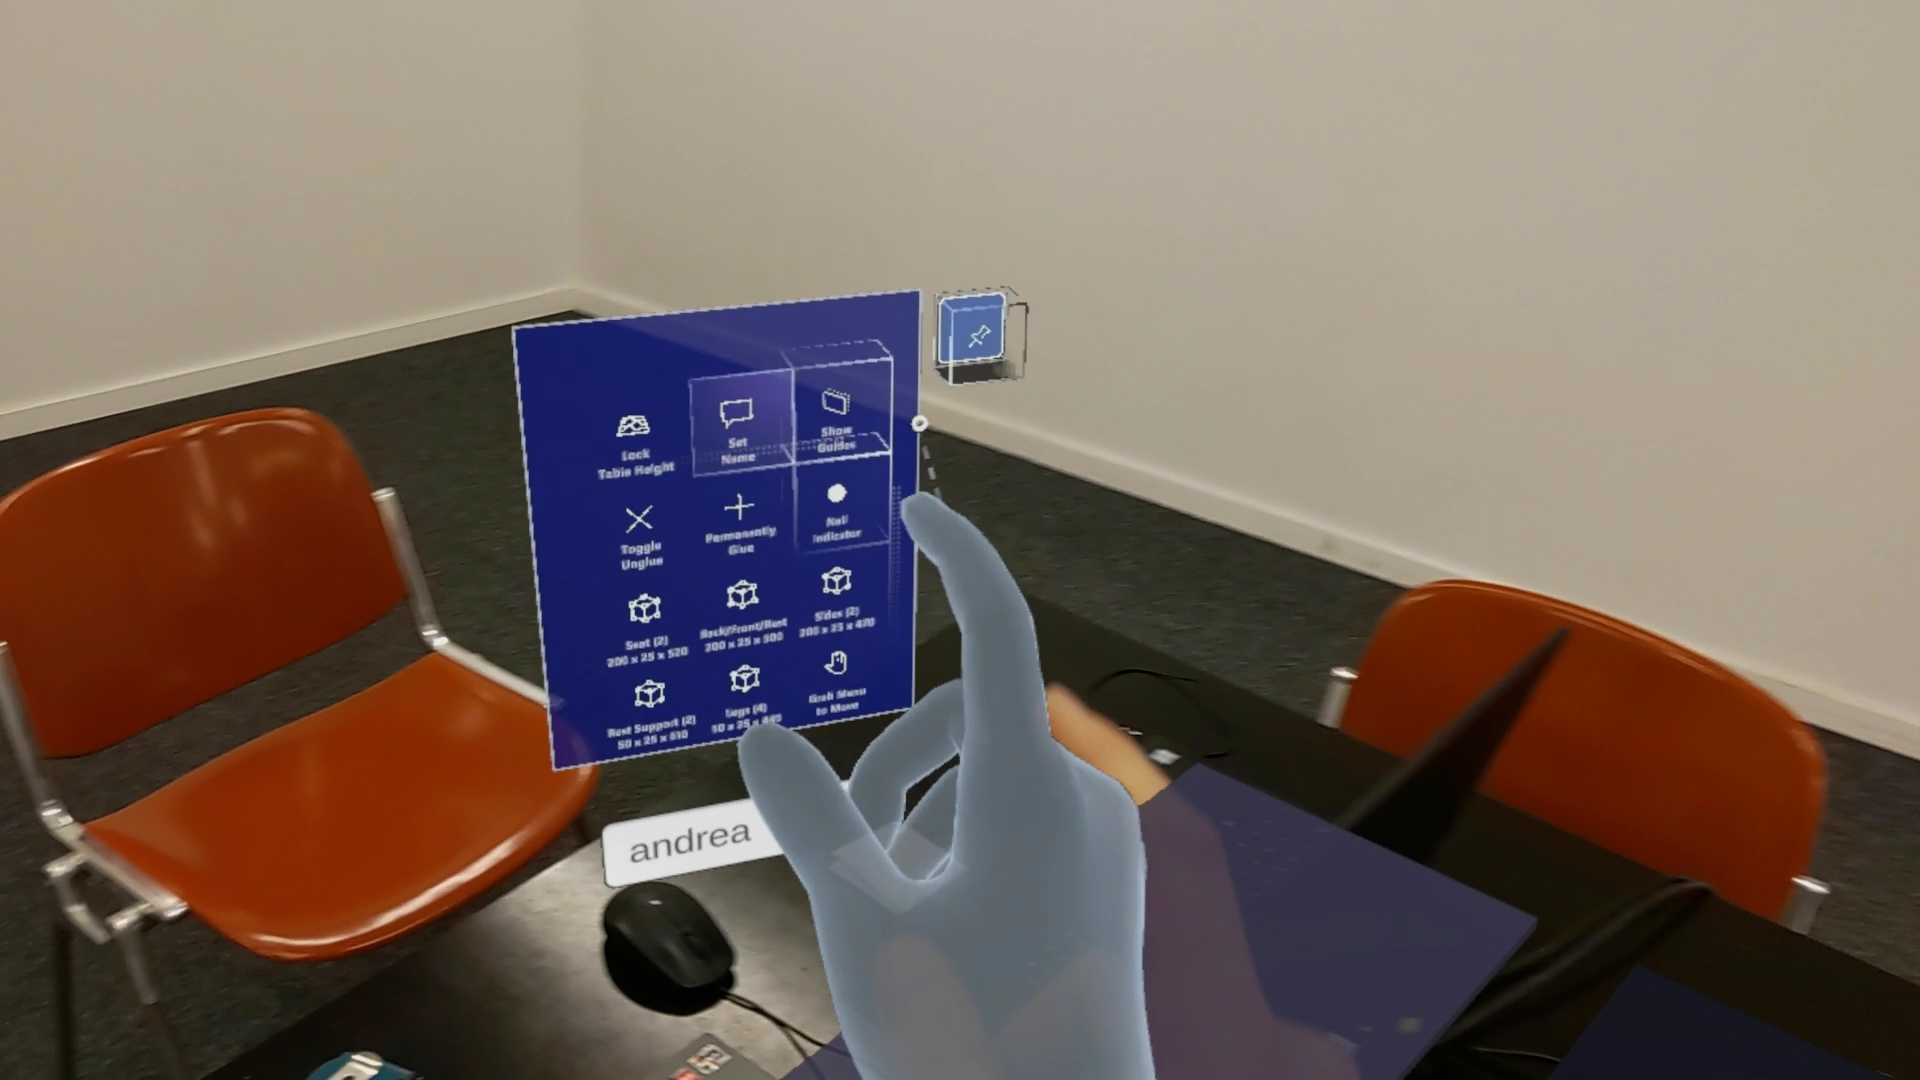
\includegraphics[width=1\linewidth]{UI2.jpg}
    \caption{UI panel. Image by the authors.}
    \label{fig:UI}
\end{figure}

For both users to focus on their tasks, we aimed to make both the user interface and overall user experience as intuitive as possible. Key elements are the common working table used to demonstrate geometries by assembling virtual objects serving as a guide for physical objects and a small floating UI panel with critical functions (see \cref{fig:UI}).

All the instantiated objects and the user avatars are made visible to all users in the room through the Photon network; their position is constantly updated in relation to the table. Nevertheless, the UI panel and the worktable can be adjusted in height, horizontal rotation, and position individually without affecting the other player's experience. This flexibility is essential because different users might be working in different room setups and orientations and sitting or standing in front of tables of varying heights. This feature is significant for the AR user, who can adjust the virtual workplace to precisely coincide with the physical workplace. After setting the table height and position, each user can lock its location using the UI menu. The menu also offers the possibility to enter and display a user's name on top of their head, select different glueing behaviors, and spawn guide objects and pointers.


\begin{figure}[!htp]
    \centering
    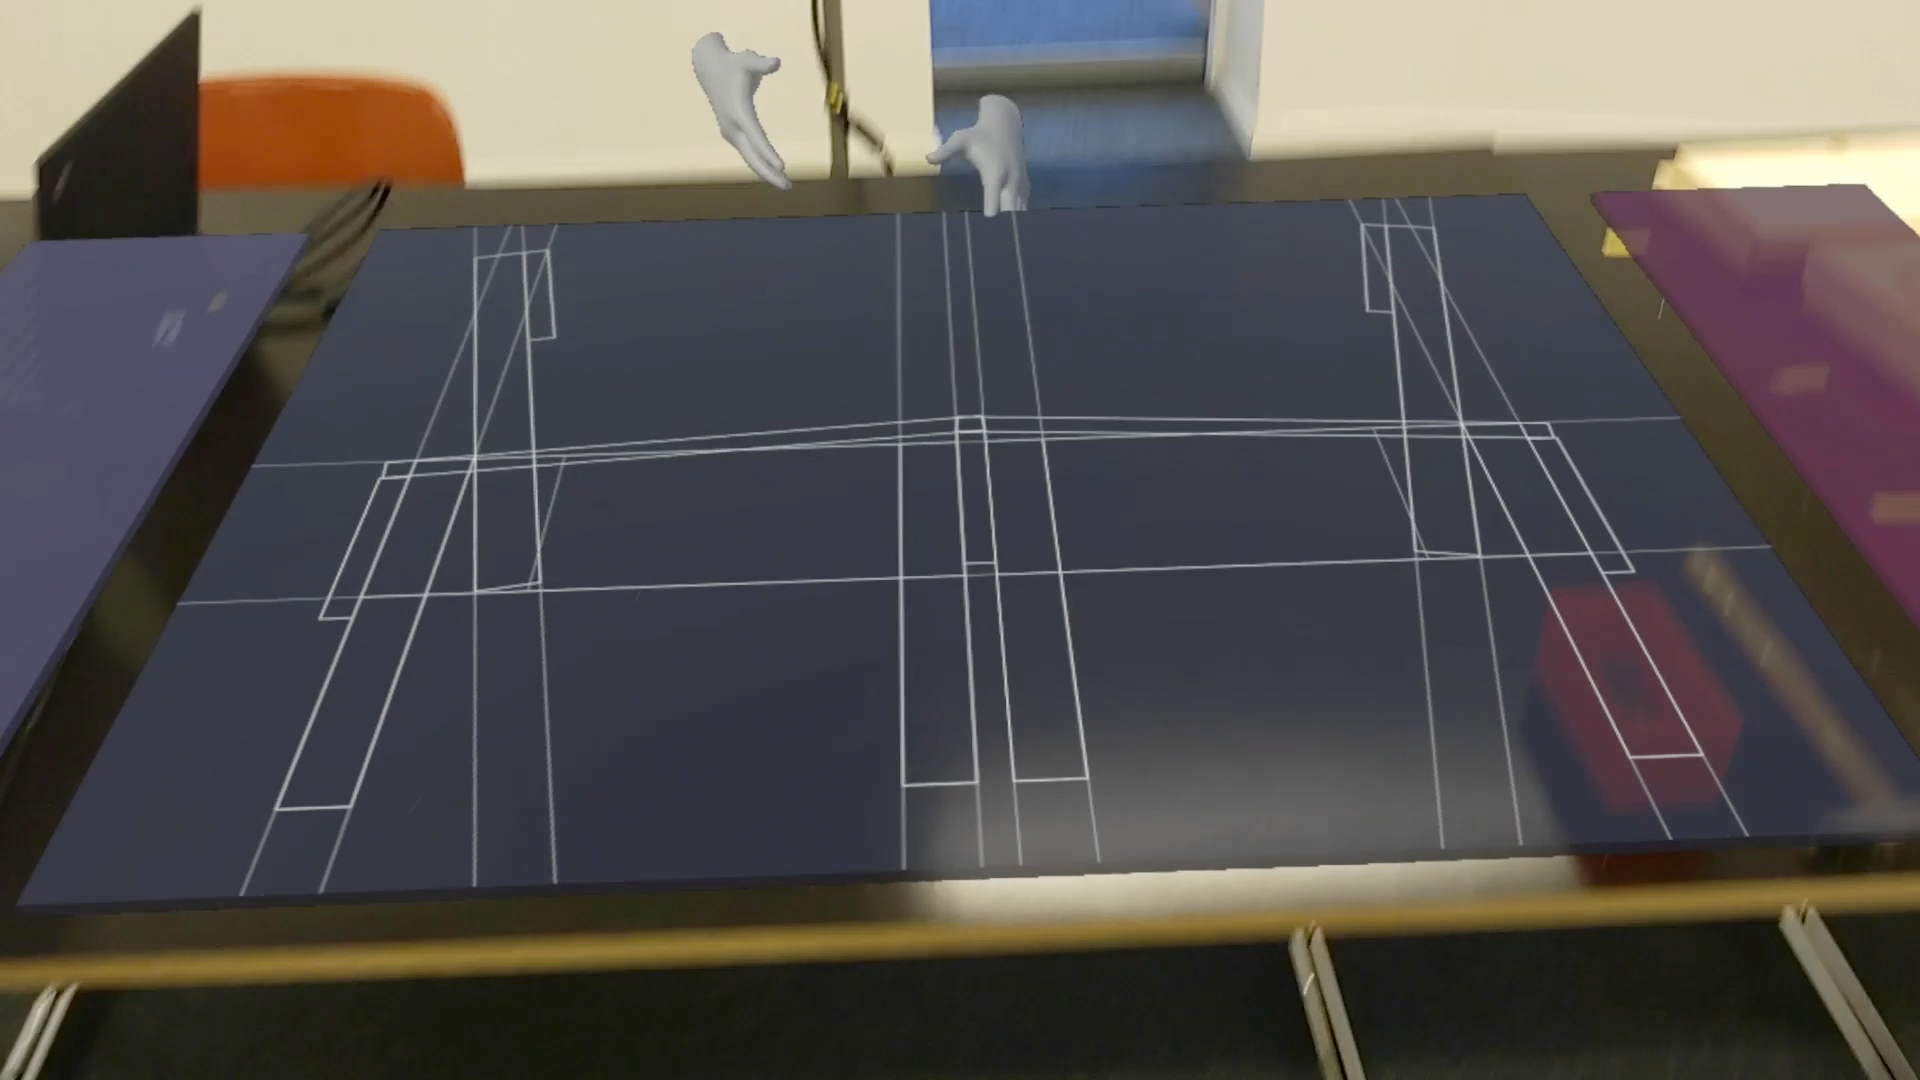
\includegraphics[width=1\linewidth]{Workplane.png}
    \caption{Work table with spawning area (left) and deletion area (right). Image by the authors.}
    \label{fig:workplane}
\end{figure}


The work table consists of three separate planes, differentiated by color (see \cref{fig:workplane}. The left blue section is where new guide objects are spawned, keeping them from interfering with the construction. The middle part of the table is the main construction plane and is sized according to the geometry to be built. Precise construction guides, indicating angles, can be toggled on and off with the UI menu. Finally, the red section of the work table destroys objects on collision.

\subsection{Guide Objects and Interaction Primitives}

\begin{figure}[!htp]
    \centering
    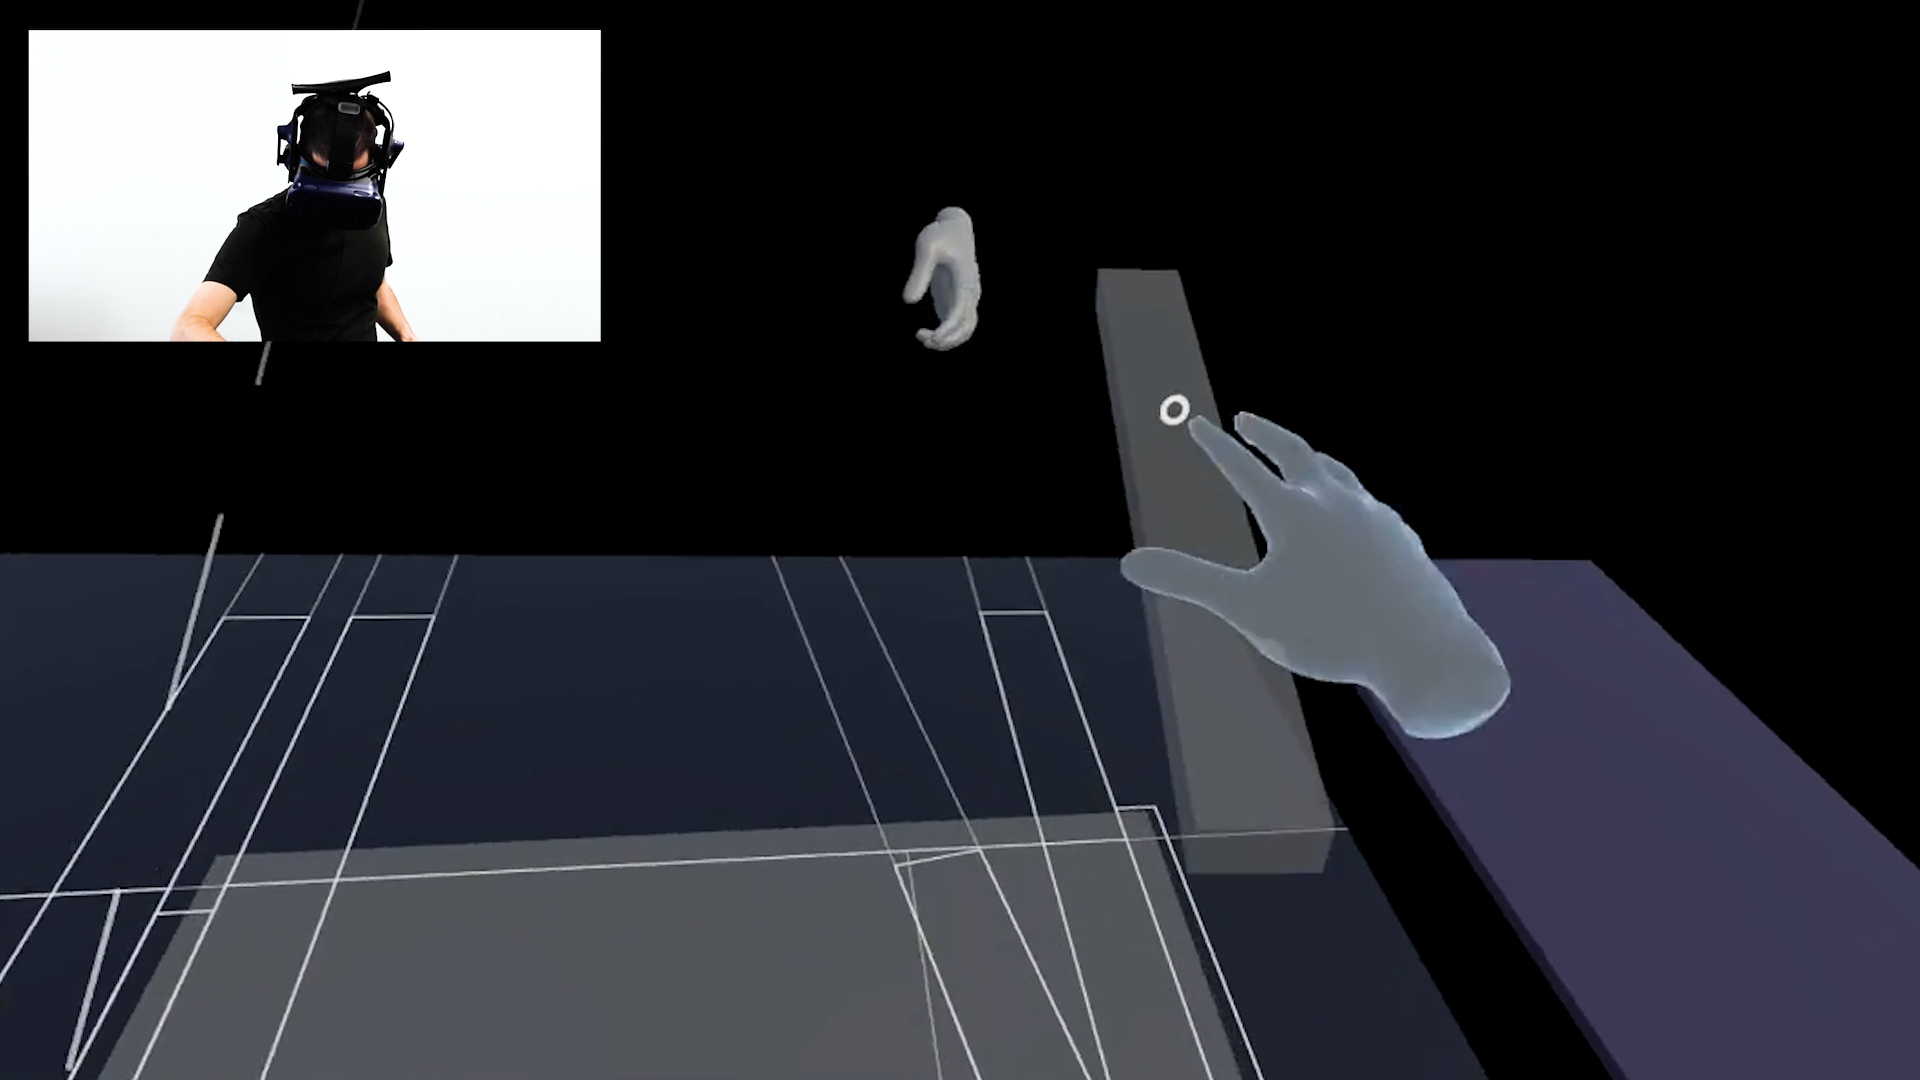
\includegraphics[width=1\linewidth]{Guide Objects.jpg}
    \caption{Placing Guide objects. Image by the authors.}
    \label{fig:Objects}
\end{figure}

Guide objects correspond to digital twins of physical counterparts, e.g.\ sections of an assemblage, machine components, or blocks of raw material. They have the same dimension in AR and VR, which makes them perfect for overlying the real and the virtual world, showing how physical elements need to be laid out, and even checking measurements of components. For our application, we designed them to have a high degree of transparency (see \cref{fig:Objects}), so that they do not obscure or irritate the AR user who sees both guide objects and real objects.

Guide objects can be spawned, manipulated and deleted by both users to allow for different collaboration scenarios. By default, a single user (i.e.\ the object owner) can modify the shared state of a networked object. To make the objects interactable for all users, we implemented an ownership transfer mechanism: Users automatically become the new owner of an object when they interact with it. 

\subsection{Gestures and Pointers}

\begin{figure}[!htp]
    \centering
    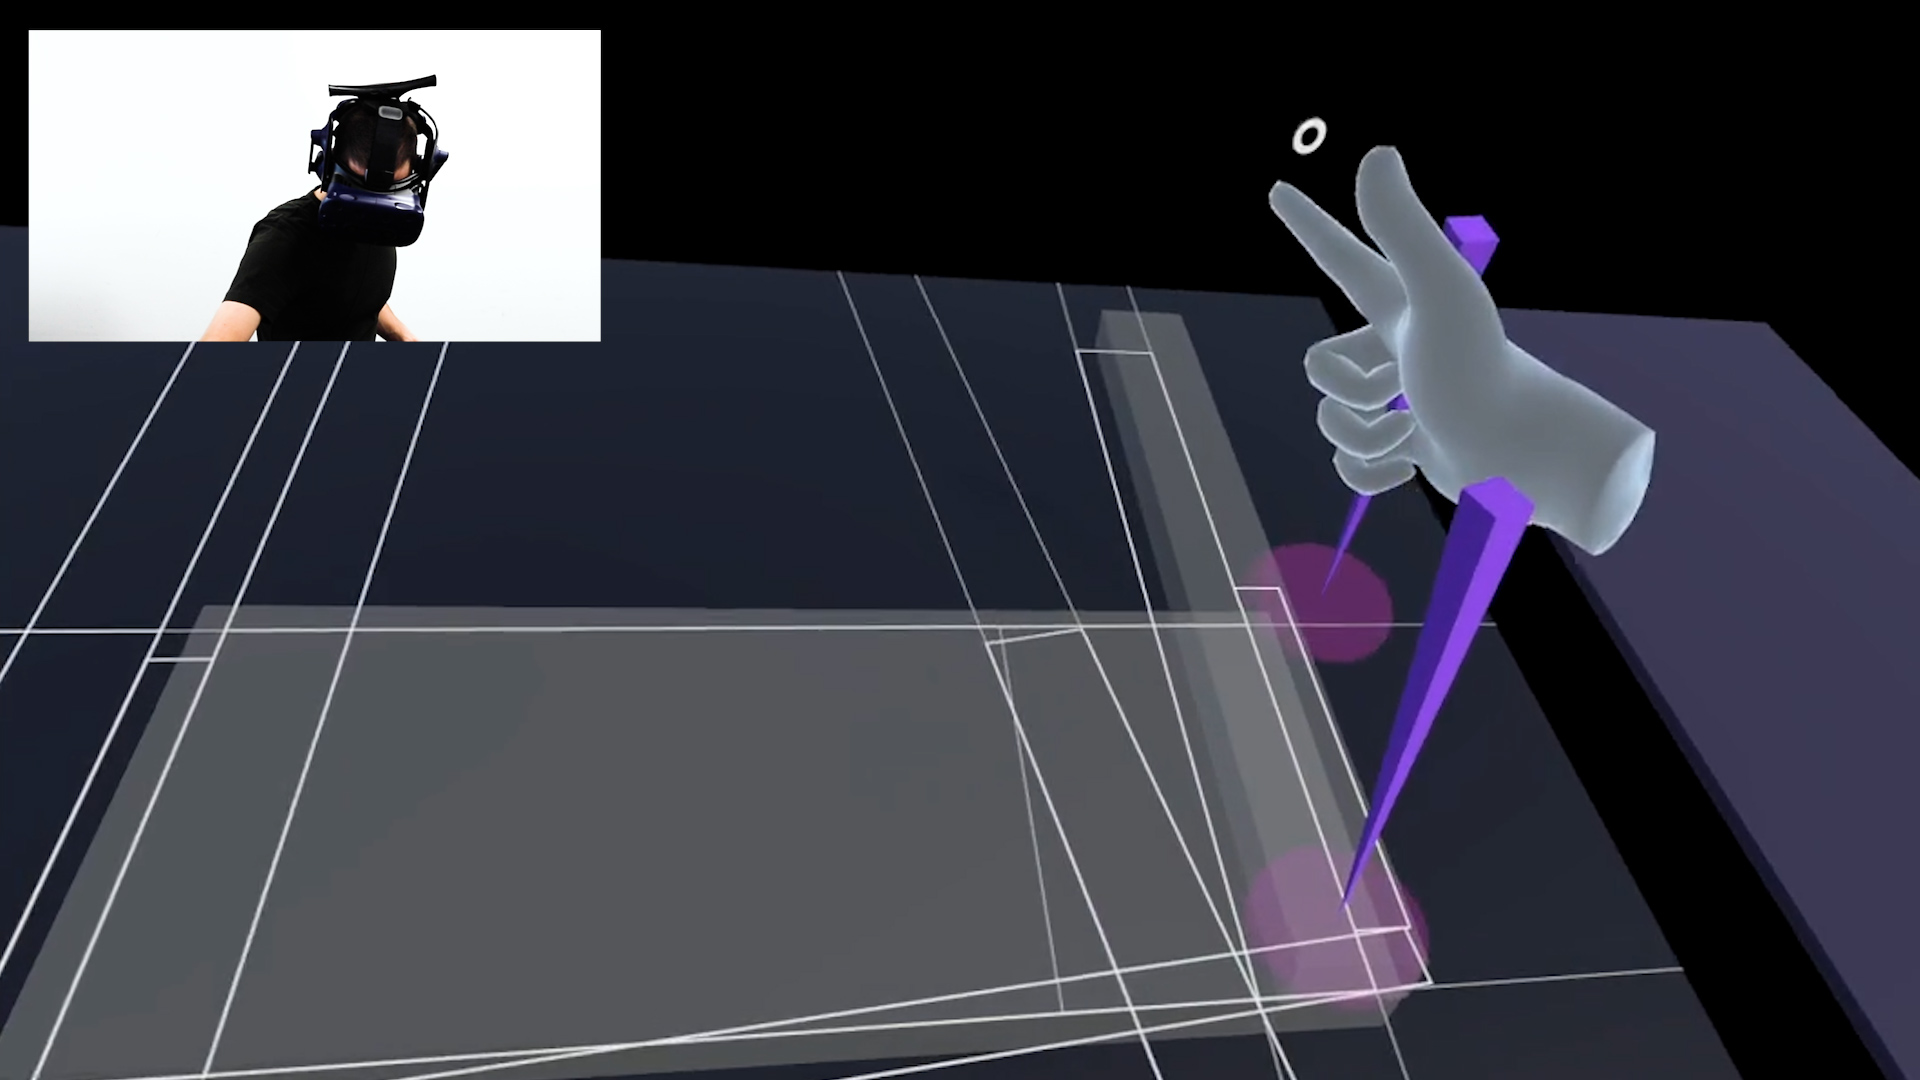
\includegraphics[width=1\linewidth]{Pointers 2.jpg}
    \caption{Pointer objects indicate nail locations. Image by the authors.}
    \label{fig:pointers}
\end{figure}

Working in MR allows moving around shared geometry and indicating exact positions in space, a task that would be cumbersome and imprecise if done by voice only. This is a key advantage of MR collaboration over conventional conversations over phone or video chat. Both AR and VR users can point to exact locations by pointing hand gestures or spawning specific pointers, which serve as precise markers on guide object assemblages (see \cref{fig:pointers}).

\subsection{Glue and Unglue Operations}

As the AR user nails chair parts together, he or she builds larger components (e.g.\ the left side of the chair), and is able to move all the parts that make up a component together. After moving this physical object, it would be inconvenient to have to move individually all the virtual parts that correspond to this component. Therefore, parts should behave as connected assemblages in the virtual world, as much as they do in the physical world when nailed together. To that end, we provided three interaction modes to the users:

\begin{enumerate}
    \item \emph{Collision mode:} Users can move the virtual parts (or group of parts) by interacting with them; all the virtual elements collide so as to avoid part inter-penetration.
    \item \emph{Glue mode:} Users can move the virtual parts (or group of parts) by interacting with them; however, upon collision, two parts are ``glued'' into a group of parts and can now only be moved together. Similarly, two groups of parts can also be glued together into a single group of parts.
    \item \emph{Unglue mode:} Users can move the virtual parts by interacting with them. Interacting with a part that is glued will ``unglue'' it, thus making it independent again.
\end{enumerate}

\begin{figure}[!htp]
    \centering
    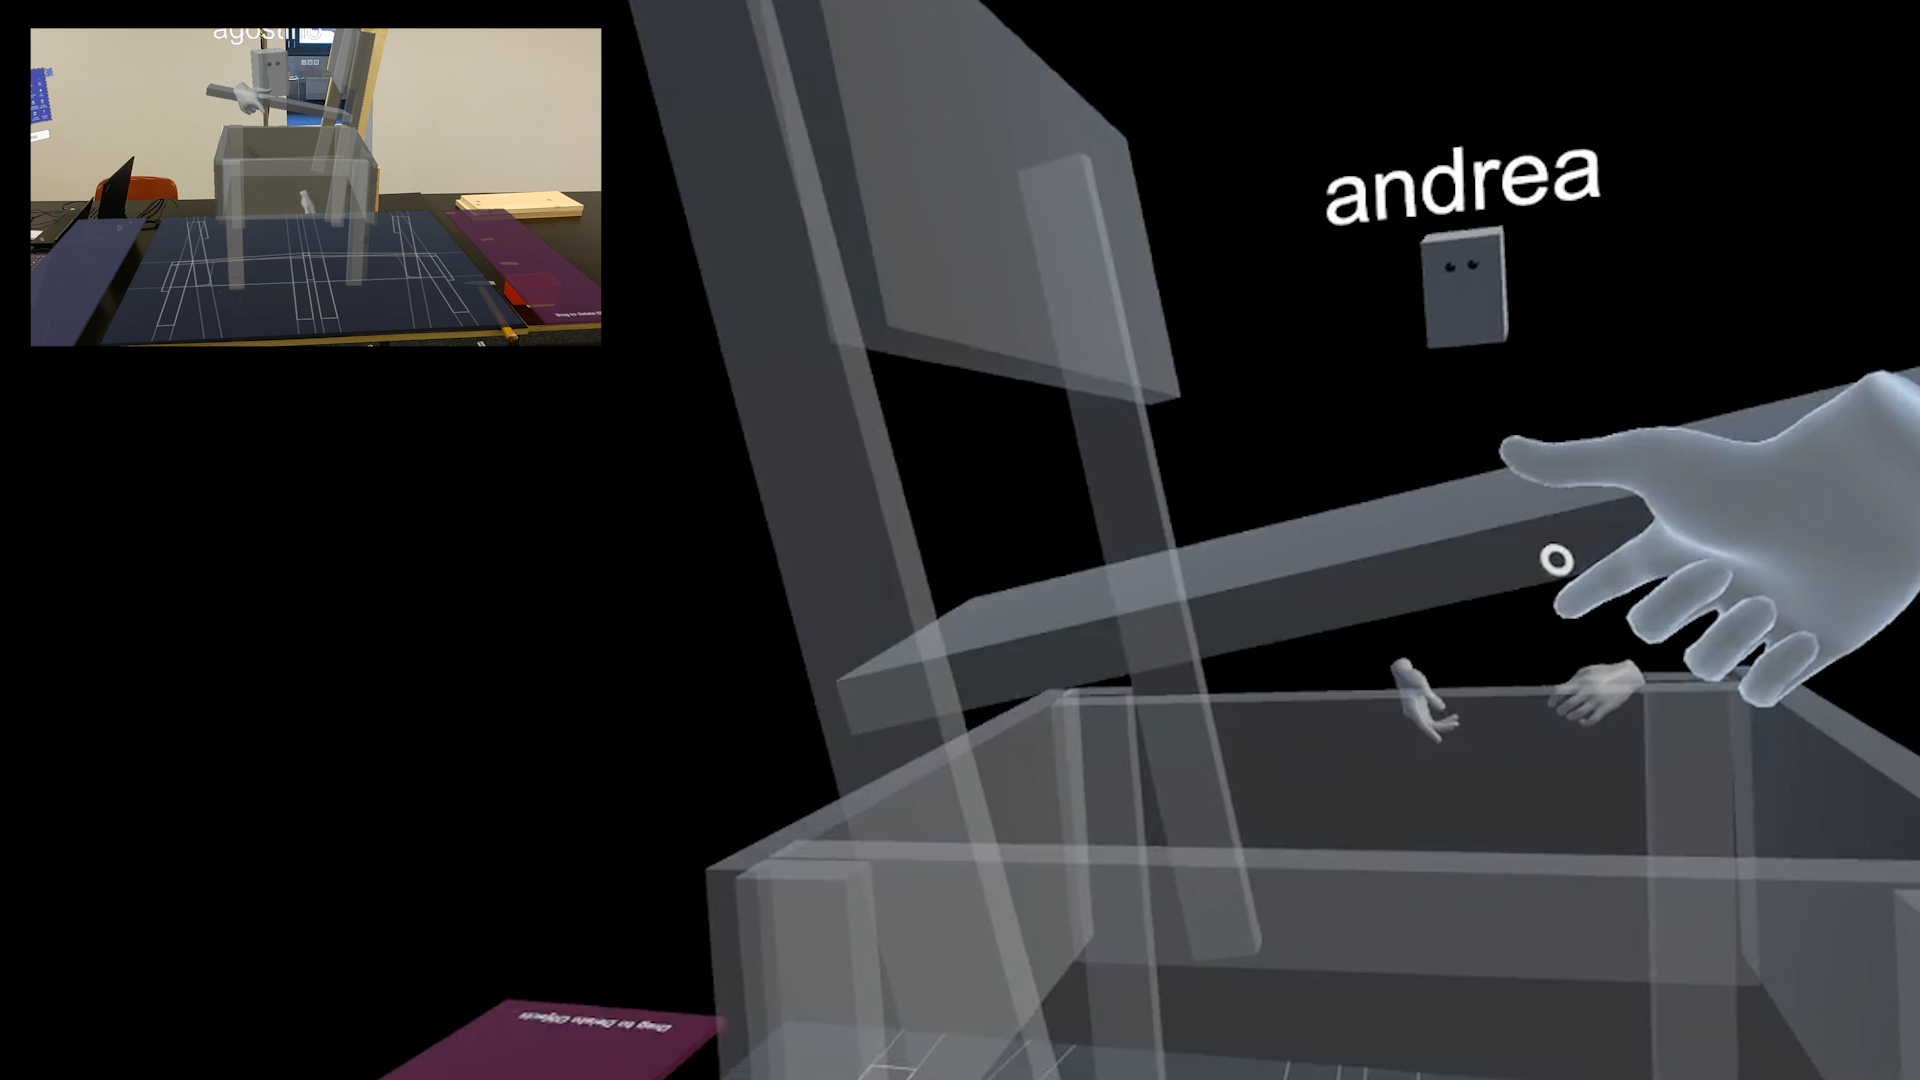
\includegraphics[width=1\linewidth]{Complex.jpg}
    \caption{Complex chair assemblage enabled by glueing. Image by the authors.}
    \label{fig:Glue}
\end{figure}


These three modes already enable to build the chair incrementally in a hierarchical manner (e.g.\ build the left side, then the right side, then connect them together). It also helps fix improper glueing of parts or improper positioning within a group when a user unintentionally makes two objects collide in glue mode.

However, having only these three modes would still be too limiting: If we imagine a situation in which users make the left side and the right side of the chair (each made up of several parts) collide to glue them together, but glue them incorrectly, they would have to unglue all the parts that make the right side individually, to fix their mistake. To solve this problem, we added an option to ``permanently glue'' the existing components. For instance, the user would press the ``permanently glue'' button right after building the left side, and another time after building the right side. If the user improperly glues the right side to the left side and switches to unglue mode, she or he can now unglue the whole right side in one go (but loses the ability to unglue the parts that make up the right side-–as would be the case if parts would actually be nailed together).

This functionality is implemented by building up trees representing the group of parts that are glued together: The leaves of the tree correspond to chair parts, the other nodes correspond to glueing operations. All the parts under a common root node are glued together. When two components collide, their corresponding trees are merged under a common root node. When ungluing a component, the subtree corresponding to that component is moved back into a stand-alone tree.

\section{Evaluation}

\begin{figure}[!htp]
    \centering
    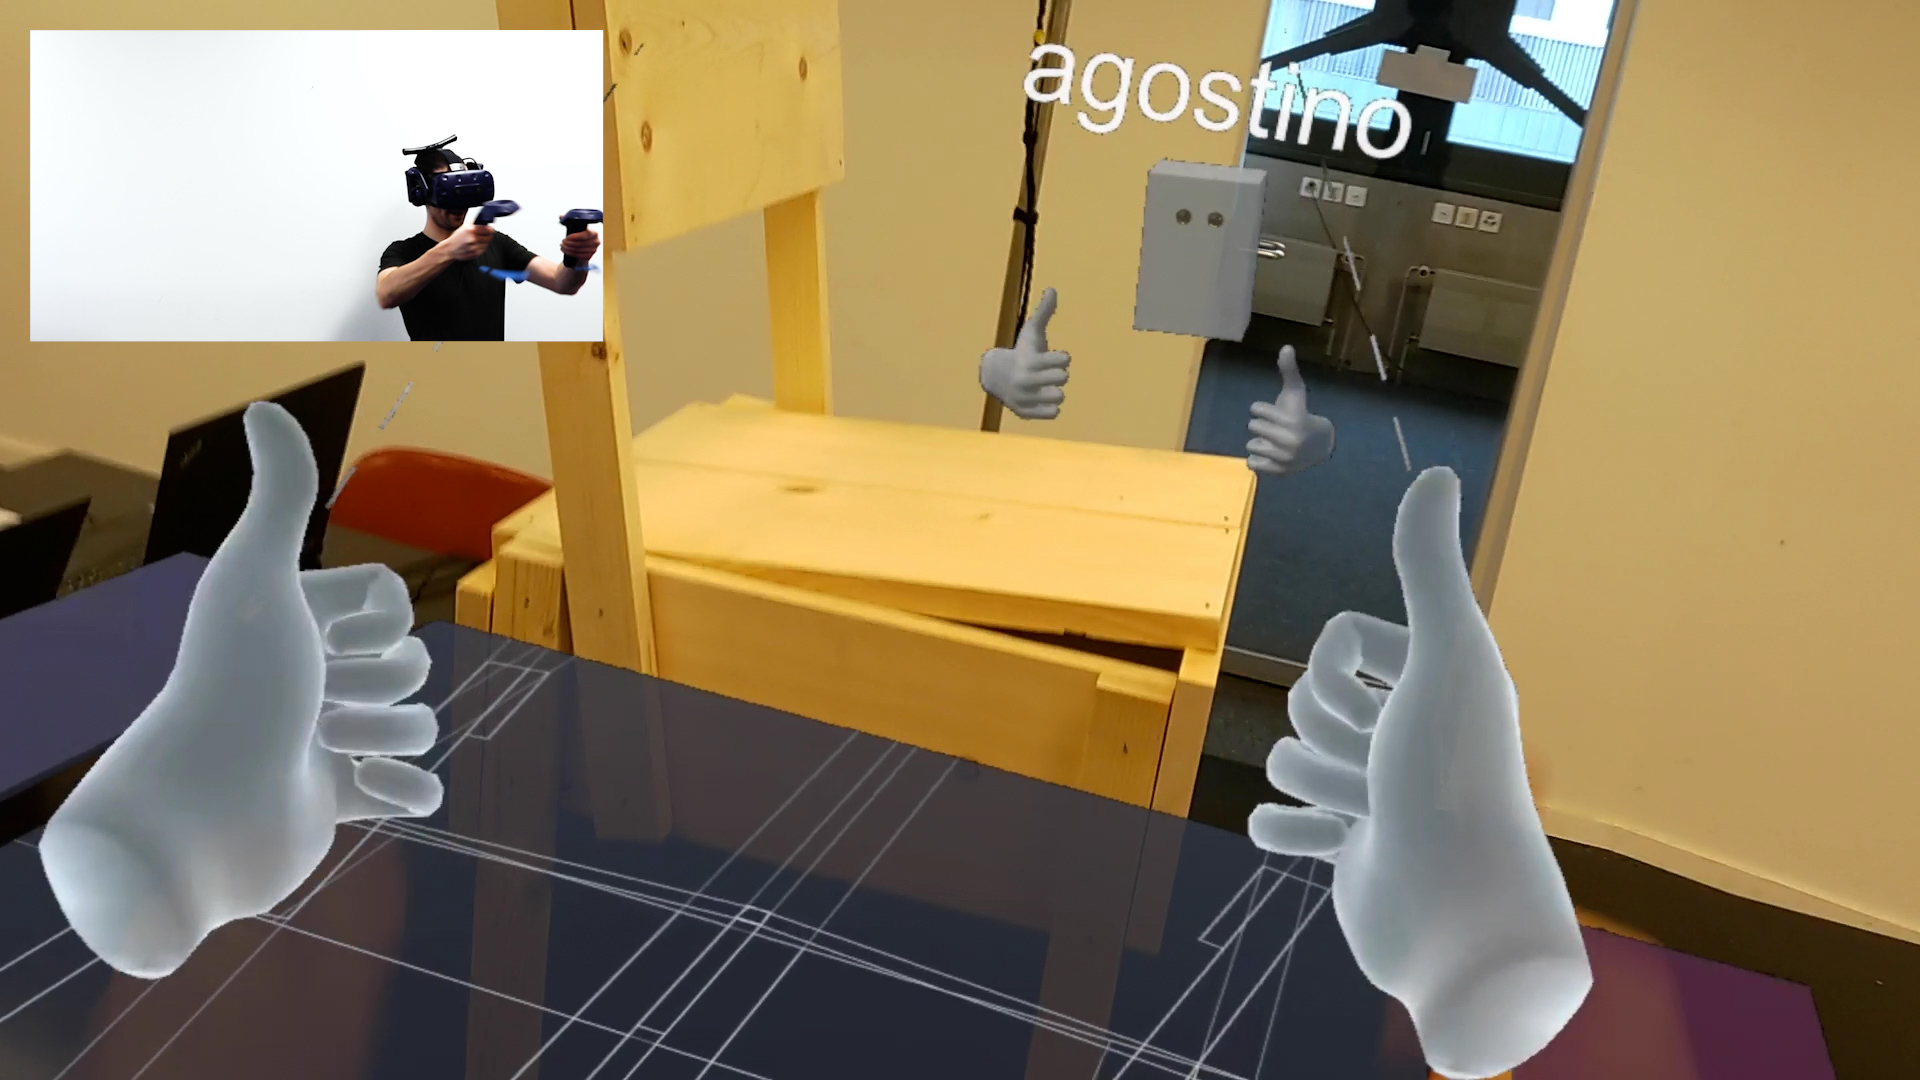
\includegraphics[width=1\linewidth]{Finished.jpg}
    \caption{End of AR/VR collaboration. Image by the authors.}
    \label{fig:Finished}
\end{figure}

In a test run, the collaborative platform allowed to fully guide an operator during the assembly of a chair. It showed that it is possible to perform a fairly complex assembly without the need for paper instructions or physical markings. Thanks to the instructions shared intuitively over voice chat, with embodied avatars and guide objects, the AR user was perfectly able to replicate the step-by-step virtual stimuli without encountering major problems. The Hololens's hands-free interface and user input system based on hand tracking resulted as particularly suitable for assembly application as the one presented here.


\section{Limitations}

The scope of our project was intentionally very limited so as to make development manageable. Additionally, evaluating the program revealed a number of limitations in our project, including technical issues that could be fixed by improving the application, design issues that hinder the user experience, or more fundamental issues with our approach or with the state of the AR/VR ecosystem.

The most prominent intentional limitation of our application is that it is highly specialized: It currently only provides the building blocks and the blueprint necessary to build a specific model of chair, and does not make it easy to add other building blocks or blueprints.

\paragraph{}
On the technical side, as has been noted earlier in this report, we encountered two bugs in MRTK while developing the application. While the first one, relating to how toggling collisions on and off on an element would disable hand interaction, could be worked around, the second one still prevents our application from being used normally on the HTC Vive: The controller tracking on the HTC Vive, when using the OpenXR deployment target, is only available in the Unity debugging mode called ``Play mode'', and not in full application builds. The technical limitation should be lifted as soon as the corresponding bug is fixed in MRTK.

Another technical issue prevents users from joining (or re-joining) after other users have started interacting with elements of the scene. Indeed, the application currently relies both on state synchronization for simple variable data, and on punctual coordinated updates on all devices for more complex modifications (e.g.\ updates of the positions of nodes in the Unity node hierarchy). A late-joiner will receive the value of the shared state, but will not carry out the punctual updates that have been initiated before she joined the network: Some elements that should be the same for all users will present different properties for this specific user.

\paragraph{}

The first limitation of our approach comes down to the user interface used to select the interaction modes and to add new virtual elements. Currently, we use one button to cycle through the interaction modes, one button per chair part for spawning, and other buttons to toggle specific functionalities in the scene (e.g.\ table alignment, blueprint, \dots). All these buttons are gathered on a single pane. This user interface was deemed uncomfortable to use. Switching between the interaction modes was found to be done very often by the users, and given the current position of the button results in a constant back-and-forth motion between the table and the button pane. The large number of buttons to add new virtual elements to the scene makes it hard to find the correct button when a new part needs to be added, and even pressing the correct button can be challenging.

A second limitation of our approach that was revealed during the evaluation is that it was not possible to completely disable interactions with virtual elements for the AR user. However, as the AR user interacts with the physical world, it was a common occurrence to unintentionally interact with virtual elements. In particular, when the user tries to actually build the chair, his or her movements (either to adjust the position of a part, or to nail it into place) would often be mistaken for attempts to grab and move the virtual parts. This option has since been added to the application, but adding it as an additional interaction mode in the menu only makes the previous limitation worse.

\paragraph{}
Finally, we also found that the controllers used by the VR user did not provide the accuracy required to comfortably manipulate the virtual elements. This is particularly problematic for our use case, as the VR user is the one in charge of most of the object manipulations, whereas the AR user only moves the virtual objects to correct their alignment with the physical objects. Accurate hand tracking on the VR headset would result in a better experience.

\section{Future Work}

We have identified a number of limitations by testing the application ourselves. However, a proper user study would make it possible to evaluate more precisely our application, and more generally the comfort of users in an AR/VR cooperation situation.

One potentially interesting interaction mode that we have not explored in this project, and that would greatly improve the user experience of the AR user, would be to make it possible to bind virtual elements to physical objects, so that the AR user can interact directly with the physical world, and have her or his modifications to the state of the elements reflected in the virtual world. While the scene understanding functionality of the Hololens 2 alone would be too limited for this task, it might be possible to tag the physical parts with ArUco markers to track their movement in space.


\section{Discussion and conclusion}

\begin{figure}[htp]
    \centering
    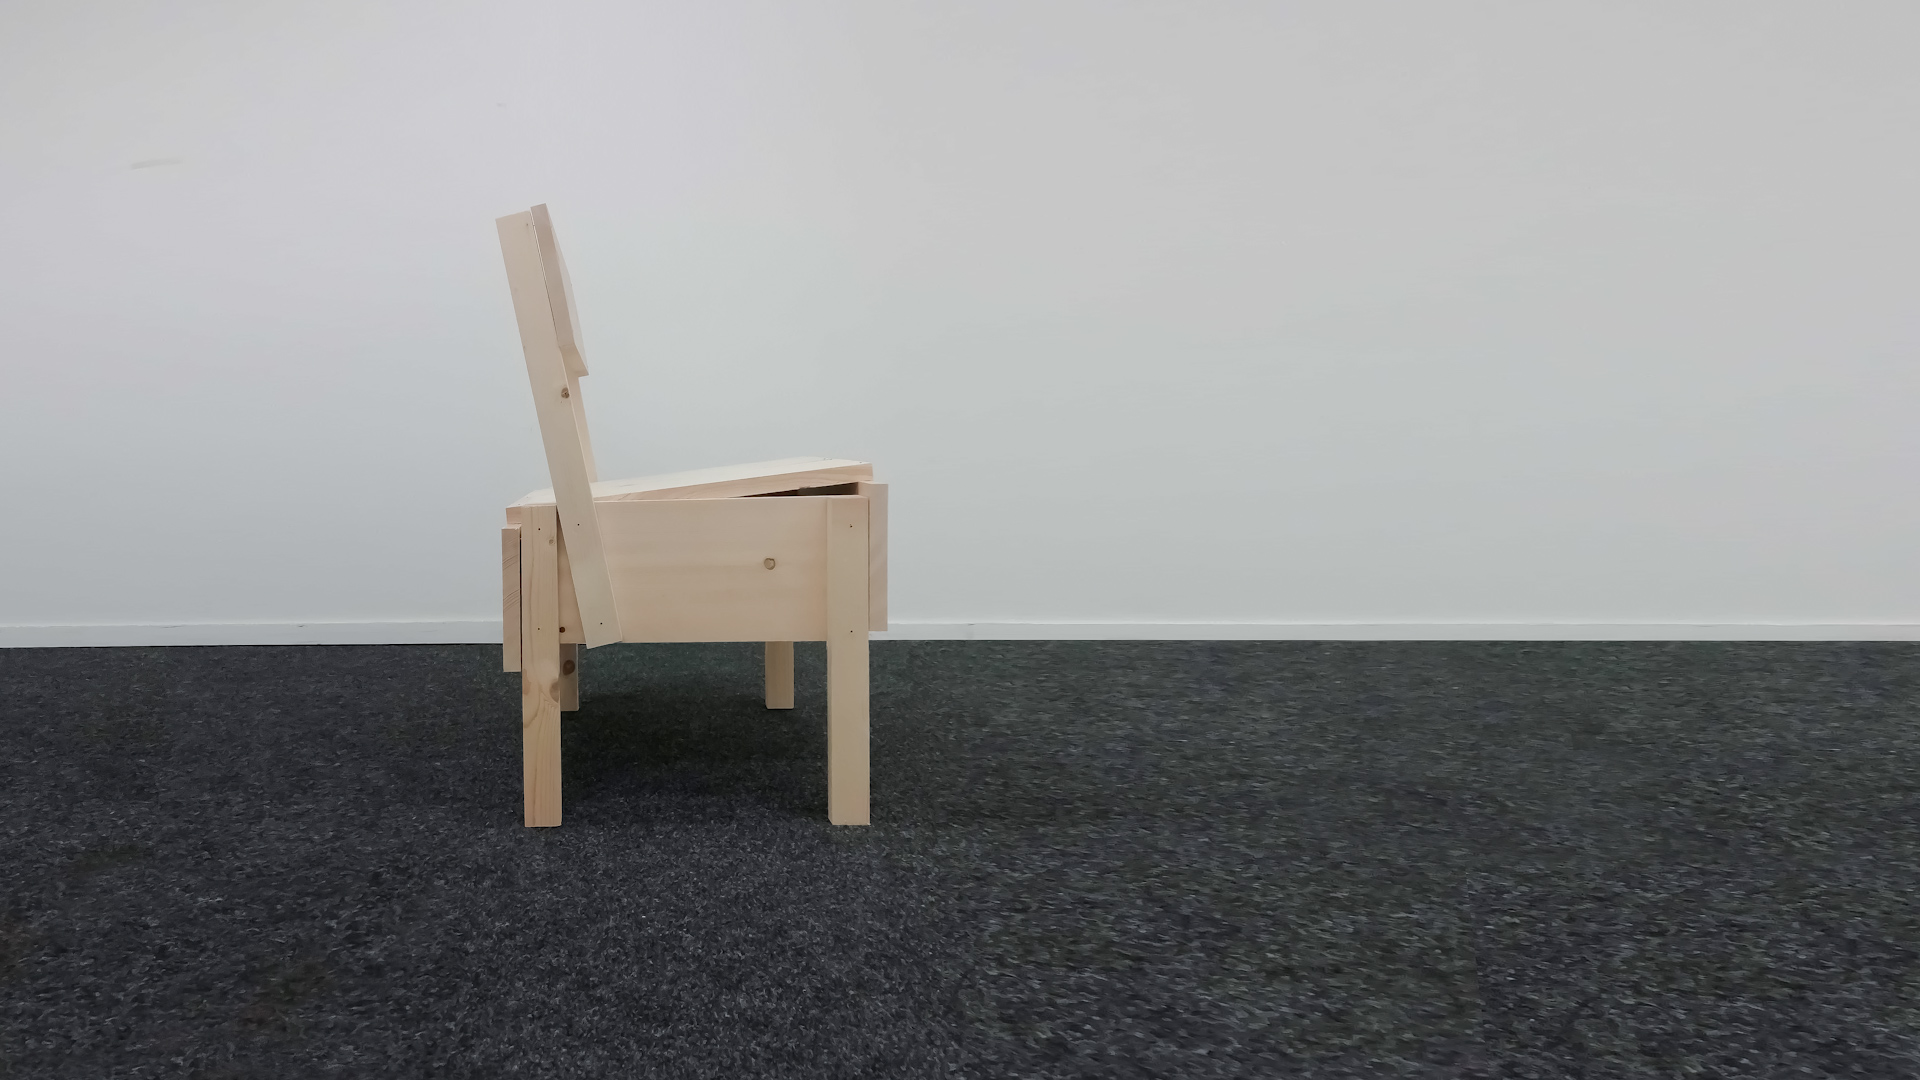
\includegraphics[width=1\linewidth]{Chair.jpg}
    \caption{The finished product. Image by the authors.}
    \label{fig:Chair}
\end{figure}

In this work, we presented a proof of concept demonstrating how AR and VR can be used together for cooperation. Our work shows that a simple networked application connecting an AR and a VR user can provide some useful features in training situations: In our demonstration, the instructor was fully able to accomplish in the virtual world the task that the trainee was trying to carry out, and thus guided the trainee and helped him learn how the task is done. We chose to evaluate the possibilities of cooperation on a very specific task, but we believe that this task is representative of many situations where AR/VR could be beneficial: Building a chair, using an industrial machine, operating on a patient are all tasks that require knowledge and dexterity and for which a trainee can learn from imitating an instructor, or from following her or his guidance. What's more, we also believe that the parts of our application that are specific to the chair building task are simple enough to be adapted or replaced for other tasks.

Nonetheless, we have noticed that the interface provided to the users, even when presented with a specific task, can become unwieldy and uncomfortable to use. In this situation, it is hard to imagine that a general-purpose application could at the same time prove useful in a large number of cooperation situations and be manageable for users. At the same time, designing AR/VR cooperation applications for every cooperation situation where they are needed would constitute a very significant engineering effort, with the risk of large amounts of duplicated work, and resulting in many undertested, potentially buggy components. An interesting middle ground that could be accomplished by breaking up our application into reusable components would be to make available a library providing networked AR/VR components, in the spirit of MRTK but with the added complexity of dealing with synchronization between several users.

\section{Demo Video\label{sec:demo_vid}}

A short demo video can be accessed \href{https://drive.google.com/file/d/1BtD-58ZoURA6vvYbpO8RtQwbVprp7i_w/view?usp=sharing}{here}.

\section{Acknowledgements}

Many thanks to our supervisors Christian Hirt and Kordian Caplazi for their support throughout the project, and to Dirk Figge from Exit Games, who shared with us the Photon voice-chat plug-in for the Hololens 2.

\bibliography{bibliography}

\end{document}
